%% LyX 2.4.3 created this file.  For more info, see https://www.lyx.org/.
%% Do not edit unless you really know what you are doing.
\documentclass[10pt,english,t,10pt,handout]{beamer}
\usepackage{lmodern}
\usepackage[T1]{fontenc}
\usepackage[utf8]{inputenc}
\setcounter{tocdepth}{1}
\usepackage{amstext}
\usepackage{amssymb}
\usepackage{graphicx}
\usepackage[authoryear]{natbib}

\makeatletter

%%%%%%%%%%%%%%%%%%%%%%%%%%%%%% LyX specific LaTeX commands.
%% Because html converters don't know tabularnewline
\providecommand{\tabularnewline}{\\}

%%%%%%%%%%%%%%%%%%%%%%%%%%%%%% Textclass specific LaTeX commands.
% this default might be overridden by plain title style
\newcommand\makebeamertitle{\frame{\maketitle}}%
% (ERT) argument for the TOC
\AtBeginDocument{%
  \let\origtableofcontents=\tableofcontents
  \def\tableofcontents{\@ifnextchar[{\origtableofcontents}{\gobbletableofcontents}}
  \def\gobbletableofcontents#1{\origtableofcontents}
}

%%%%%%%%%%%%%%%%%%%%%%%%%%%%%% User specified LaTeX commands.



\usepackage{tikz}
\usetikzlibrary{positioning}
\usepackage{appendixnumberbeamer}

\usepackage{graphicx}
\usepackage{subfig}

\usetheme[progressbar=frametitle,block=fill,subsectionpage=progressbar]{metropolis}

% margin
\setbeamersize{text margin right=1.5cm}

% colors
\definecolor{DarkRed}{rgb}{0.7,0,0}
\setbeamercolor{normal text}{fg=black}
\setbeamercolor{alerted text}{fg=DarkRed}
\setbeamercolor{progress bar}{fg=DarkRed}
\setbeamercolor{button}{bg=DarkRed}
\usepackage{booktabs}

% width of seperators
\makeatletter
\setlength{\metropolis@titleseparator@linewidth}{1pt}
\setlength{\metropolis@progressonsectionpage@linewidth}{1pt}
\setlength{\metropolis@progressinheadfoot@linewidth}{1pt}
\makeatother

% new alert block
\newlength\origleftmargini
\setlength\origleftmargini\leftmargini
\setbeamertemplate{itemize/enumerate body begin}{\setlength{\leftmargini}{4mm}}
\let\oldalertblock\alertblock
\let\oldendalertblock\endalertblock
\def\alertblock{\begingroup \setbeamertemplate{itemize/enumerate body begin}{\setlength{\leftmargini}{\origleftmargini}} \oldalertblock}
\def\endalertblock{\oldendalertblock \endgroup}
\setbeamertemplate{mini frame}{}
\setbeamertemplate{mini frame in current section}{}
\setbeamertemplate{mini frame in current subsection}{}
\setbeamercolor{section in head/foot}{fg=normal text.bg, bg=structure.fg}
\setbeamercolor{subsection in head/foot}{fg=normal text.bg, bg=structure.fg}

% footer
\makeatletter
\setbeamertemplate{footline}{%
    \begin{beamercolorbox}[colsep=1.5pt]{upper separation line head}
    \end{beamercolorbox}
    \begin{beamercolorbox}{section in head/foot}
      \vskip1pt\insertsectionnavigationhorizontal{\paperwidth}{}{\hskip0pt plus1filll \insertframenumber{} / \inserttotalframenumber \hskip2pt}\vskip3pt% 
    \end{beamercolorbox}%
    \begin{beamercolorbox}[colsep=1.5pt]{lower separation line head}
    \end{beamercolorbox}
}
\makeatother

% toc
\setbeamertemplate{section in toc}{\hspace*{1em}\inserttocsectionnumber.~\inserttocsection\par}
\setbeamertemplate{subsection in toc}{\hspace*{2em}\inserttocsectionnumber.\inserttocsubsectionnumber.~\inserttocsubsection\par}


% Automatically create vspace between items
% See: https://tex.stackexchange.com/questions/369504/beamer-vertically-stretching-level-1-list-items-in-a-nested-list-environment
%\usepackage{xpatch} 
%\xpatchcmd{\itemize}   
%	{\def\makelabel}   
%	{\ifnum\@itemdepth=1\relax      
%		\setlength\itemsep{\fill} % separation for first level    
%		\fi\def\makelabel   
%	}{}{} 
%\xpatchcmd{\enditemize}   
%	{\endlist}   
%	{\endlist\ifnum\@itemdepth<2\else\vfil\fi}{}{}



\newenvironment{wideitemize}{\itemize\addtolength{\itemsep}{10pt}}{\enditemize}
% Added by lyx2lyx
\setlength{\parskip}{\smallskipamount}
\setlength{\parindent}{0pt}

\makeatother

\usepackage{babel}
\begin{document}
\title{6. Wealth Inequality \vspace{-2mm}}
\subtitle{Adv. Macro: Heterogenous Agent Models} 
\author{Jeppe Druedahl, Raphaël Huleux}
\date{2024}

{
\setbeamertemplate{footline}{} 
\begin{frame}

\maketitle

\end{frame}
}

\addtocounter{framenumber}{-1}


\section{Introduction}
\begin{frame}{Wealth inequality}
\vspace{-2mm}
\begin{itemize}
\item <+->\textbf{Goal for today:} Better understand wealth inequality
through the lens of heterogeneous agent general equilibrium models
\item <+->\textbf{Central economic questions:} 
\begin{enumerate}
\item Why are some people rich while others are poor? 
\item To what extent can governments affect inequality? 
\begin{itemize}
\item What does the baseline Aiyigari model predict in terms of wealth inequality?
\item How can we augment the baseline model to obtain a closer match of
reality? 
\end{itemize}
\item What explains the rise in wealth inequality in recent decades? 
\end{enumerate}
\item <+->To answer these questions, we need to better understand why people
save, and how this translates into wealth inequality 
\item <+->\textbf{Plan for today:} 
\begin{enumerate}
\item Study the predictions of a baseline Bewley-Huggett-Aiyagari model 
\item Consider various model extensions that help match the data 
\item Given such a model, what can we say about optimal wealth taxation?
\end{enumerate}
\end{itemize}
\end{frame}
%

\section{Wealth inequality in the data}
\begin{frame}{Earnings and wealth inequality}
\begin{itemize}
\item US data on distribution of income and wealth (SCF, 1989)
\end{itemize}

\pause{}

\pause{%
\begin{tabular}{lccccc}
\hline 
 & \quad{}\quad{} & \quad{}\quad{} & \quad{}\quad{} & \quad{}\quad{} & Percent at zero\tabularnewline
 & Top $1\%$ & Top $5\%$ & Top $20\%$ & Top $40\%$ & or negative\tabularnewline
\hline 
Wealth & 29 & 53 & 80 & 93 & 6\tabularnewline
Earnings & 6 & 19 & 48 & 72 & 8\tabularnewline
\hline 
\end{tabular}}

\pause{}
\begin{itemize}
\item Wealth more concentrated than earnings
\item Skewed distributions with thick upper tails
\end{itemize}
\end{frame}
%
\begin{frame}{Wealth more concentrated than earnings}

Not only in the US, but also Denmark and almost all other countries

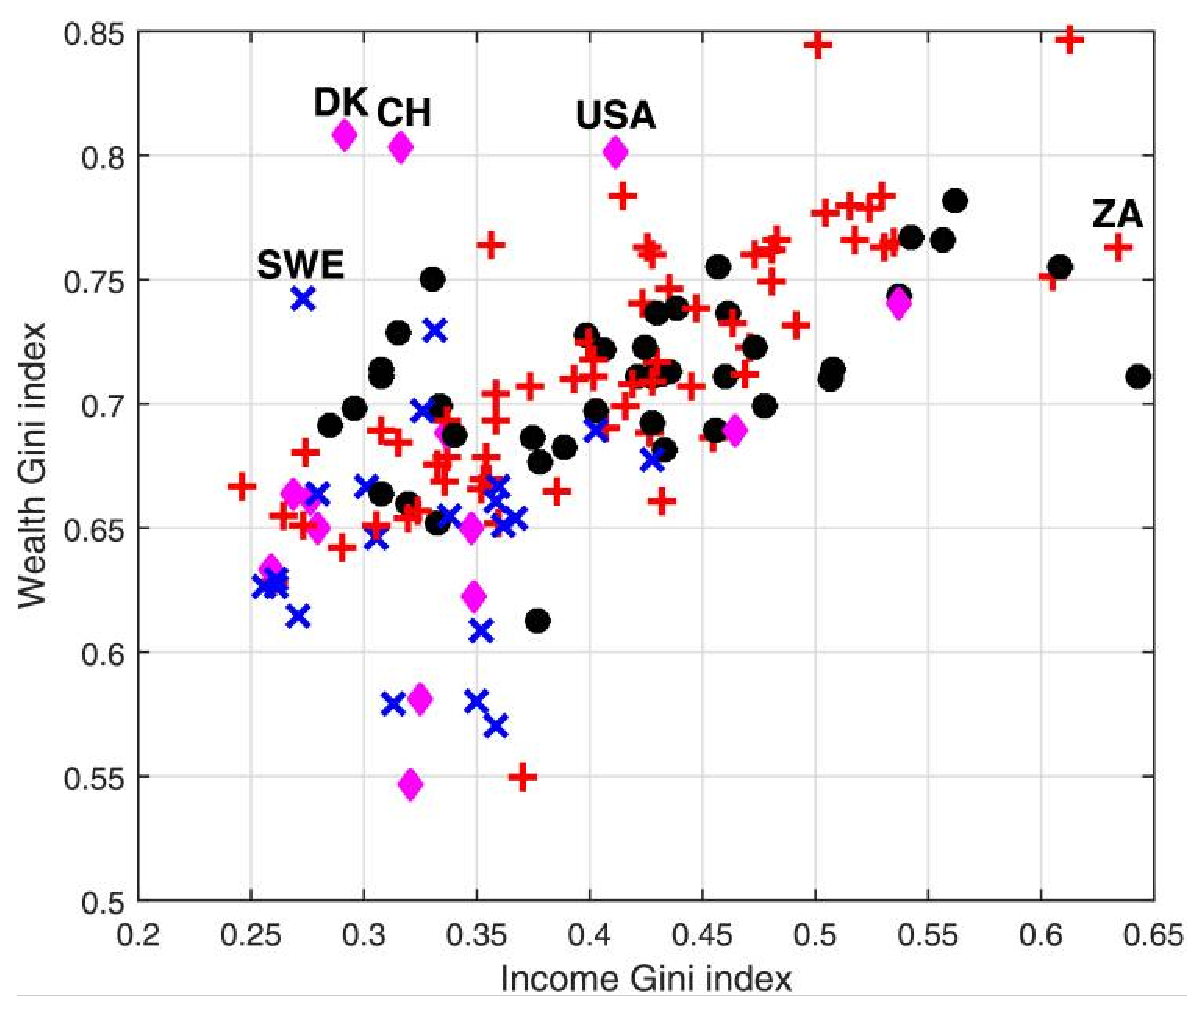
\includegraphics[width=0.75\textwidth]{figs/Cross-Country-Gini.eps} % Figure from https://www.ncbi.nlm.nih.gov/pmc/articles/PMC4841595/
\end{frame}

\begin{frame}{Top wealth shares in the US over time}

\begin{figure}
    \centering
    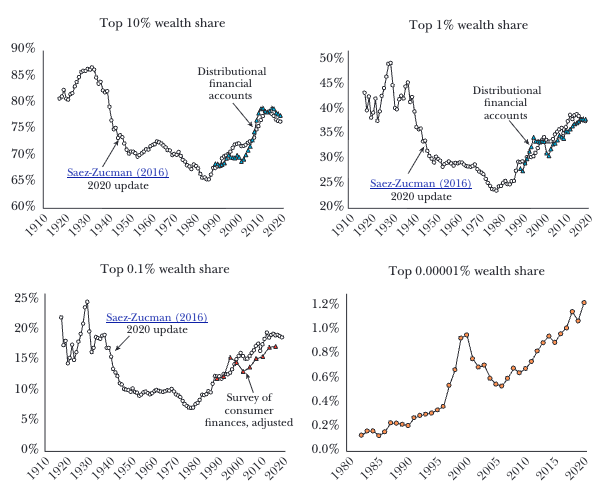
\includegraphics[width=0.9\linewidth]{figs_papers/wealth_shares_US_Saez_Zucman_2020.png}
    \caption{Figure 2 from Saez, Zucman (2020)}
\end{figure}
\end{frame}

\begin{frame}{Income inequality has increased since the 70s (US)}
\begin{figure}
        \centering
        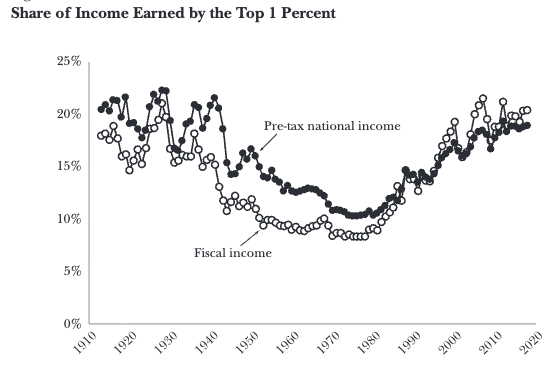
\includegraphics[width=\linewidth]{figs_papers/saez_zucman_top_1_income.png}
        \caption{Figure 3 from Saez, Zucman (2020)}
    \end{figure}
        
\end{frame}
\begin{frame}{Income growth by decile in the U.S.}
\begin{figure}
        \centering
        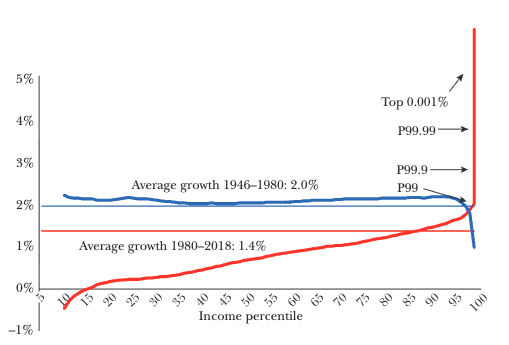
\includegraphics[width=0.75\linewidth]{figs_papers/Saez_zucman_2020_income_growth_percentile.png}
        \caption{Figure 4 from Saez, Zucman (2020)}
    \end{figure}
        
\end{frame}

\begin{frame}{Average tax rates by income groups}

\begin{figure}
        \centering
        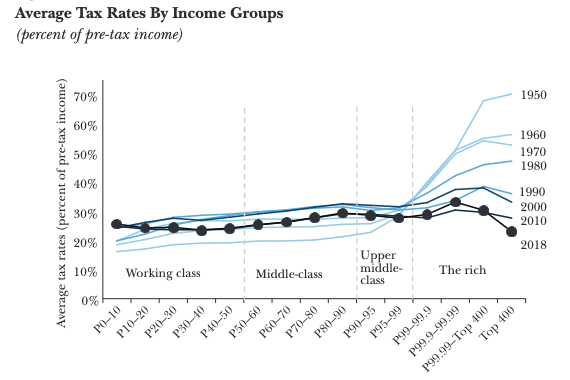
\includegraphics[width=\linewidth]{figs_papers/saez_zucman_tax_rates_income_group.png}
        \caption{Figure 5 from Saez, Zucman (2020)}
    \end{figure}    
\end{frame}

\begin{frame}{Richer households hold more risky assets}
\vspace{1cm}
\begin{figure}
    \centering
    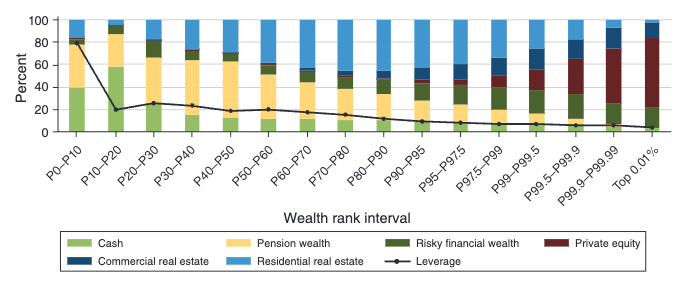
\includegraphics[width=\linewidth]{figs_papers/bach_et_al_fig_2_allocation_gross_wealth.png}
    \caption{Figure 2 from Bach et al (2020)}
\end{figure}
\end{frame}

\begin{frame}{Richer households have higher returns}
    \begin{figure}
        \centering
        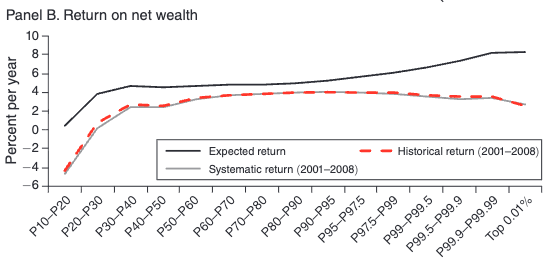
\includegraphics[width=\linewidth]{figs_papers/bach_et_al_return_net_wealth.png}
        \caption{Figure 3 from Bach et al (2020)}
    \end{figure}
$\to$ But still a debate in the literature: is it because of higher risk or higher skill (Fagereng et al, 2020)?
\end{frame}

\begin{frame}{The rich save more, because of capital gains}
\begin{figure}
        \centering
        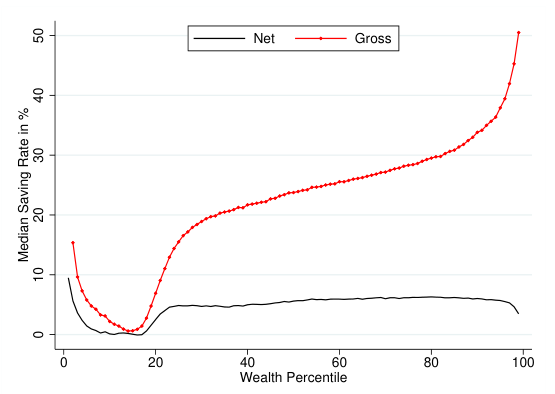
\includegraphics[width=0.75\linewidth]{figs_papers/fagereng_2020_savings_rate_capital_gains.png}
        \caption{Figure 1 from Fagereng et al (2019)}
    \end{figure}    
\end{frame}

\begin{frame}{Taking stock}
\vspace{1cm}
\begin{itemize}
    \item Wealth inequality is higher than income inequality \pause
    \item Both wealth and income inequality have increased over time \pause
    \item Taxes became less progressive over time (at least in the US) \pause
    \item Returns are heterogeneous, and higher for richer households \pause 
    \item The rich save more, mostly because of capital gains
\end{itemize}    
\end{frame}



\section{Explaining wealth inequality }

\begin{frame}{Aiyagari Model}

\begin{itemize}
\item Infinitely lived agents with preferences
\end{itemize}
\[
\max_{\left\{ c_{t}\right\} _{t=0}^{\infty}}E\sum_{t=0}^{\infty}\beta^{t}\frac{c_{t}^{1-\sigma}}{1-\sigma}
\]
\begin{itemize}
\item Budget constraint and borrowing constraint
\end{itemize}
\[
a_{t}=y_{t}+(1+r)a_{t-1}-c_{t},\quad a_{t}\geq\underline{a}
\]
\begin{itemize}
\item Idiosyncratic earnings risk:
\[
\ln y_{t}=\rho\ln y_{t-1}+\epsilon_{t},\quad\epsilon_{t}\sim\mathcal{N}\left(0,\sigma_{\epsilon}^{2}\right)
\]
\item As usual, calibrate parameters in earnings process $\left(\rho,\sigma_{\epsilon}^{2}\right)$
based on estimates from panel data on earnings, i.e. Floden and Linde
(2001)
\end{itemize}
\end{frame}
%
\begin{frame}{Aiyagari Model - wealth inequality fit}
\vspace{1cm}
\begin{center}

\begin{tabular}{lcccc}

\hline 
 & \text { Wealth Gini } & \multicolumn{3}{l}{\text { Wealth in top (\%) }}\tabularnewline
 &  & 1\% & 5 \% & 20 \%\tabularnewline
\hline 
\text { U.S. data, } 1989 \text { SCF } &  &  &  & \tabularnewline
 & .78 & 29 & 53 & 80\tabularnewline
\text { Aiyagari Baseline } &  &  &  & \tabularnewline
 & .38 & 3.2 & 12.2 & 41.0\tabularnewline
\hline 
\end{tabular}
\end{center}
\end{frame}
%
\begin{frame}{Top wealth inequality}
\begin{itemize}
\item <+->What about top wealth inequality?
\begin{itemize}
\item Think top 0.01\% or 0.001\% (Bezos,Musk, Gates etc.)
\end{itemize}
\item <+->The probability of having wealth $a$ above threshold $X$ described
as Pareto dist, $P\left(a>X\right)\sim x^{-\alpha}$
\begin{itemize}
\item In logs, $\ln P\left(a>X\right)\sim-\alpha\ln x$, so linear in log wealth
with $\alpha$ describing the "thickness of the tail"
\end{itemize}
\visible<3->{
\begin{figure}[H]     
\centering      
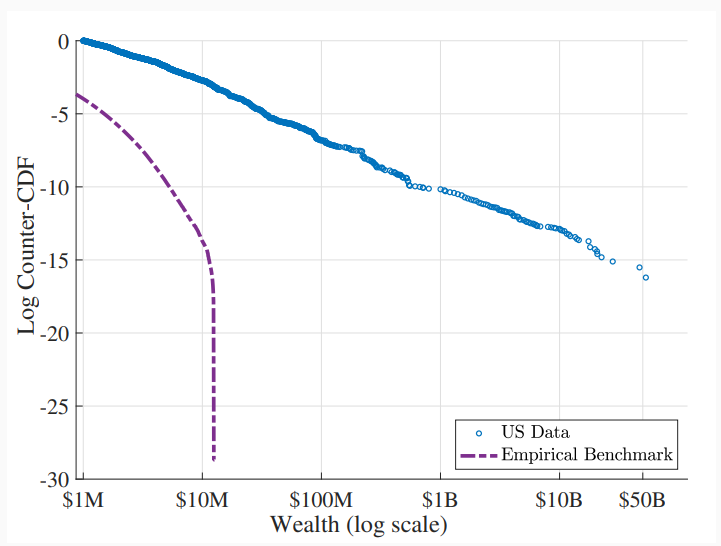
\includegraphics[width=0.5\linewidth]{figs_papers/pareto.png}      
\end{figure}
}
\end{itemize}
\end{frame}

\begin{frame}{Policies in the Buffer-Stock model}
\vspace{1cm}
\begin{figure}
    \centering
    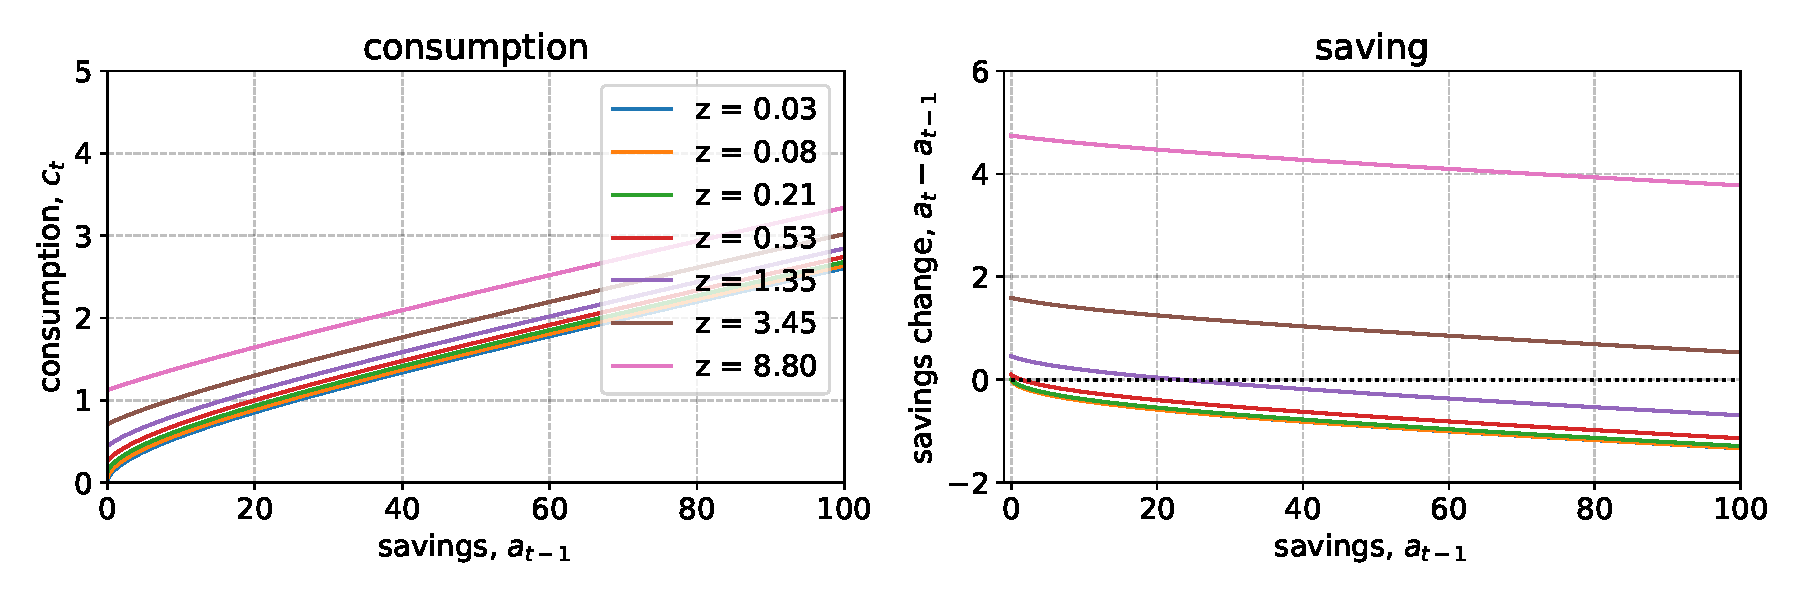
\includegraphics[width=\linewidth]{figs_papers/policy_functions_standard_model.pdf}
\end{figure}
\end{frame}
\begin{frame}{Key mechanism}
\begin{itemize}
\item <+->Precautionary savings behavior. People save to self-insure against
earnings risk
\item <+->Once buffer stock savings is reached, people start dissaving
(Carroll 1997)
\item <+->In the model: The saving rate of the high wealth households is
low or even negative
\begin{itemize}
\item Contrasts with much empirical evidence (Dynan Skinner and Zeldes,
2004 and De Nardi, French and Jones, 2010) 
\item Will discuss this in next lecture 
\end{itemize}
\item <+->Note also: Only driver of wealth inequality is earnings risk
\begin{itemize}
\item Income inequality in data typically lower than \emph{wealth} inequality
\item In reality multiple drivers such as entrepreneurship, preferences,
bequests, return heterogeneity 
\end{itemize}
\end{itemize}
\end{frame}

\begin{frame}{Explanations}
\begin{itemize}
\item <+->Standard Aiyagari model: Income inequality 
\item <+->Preference heterogeneity
\begin{itemize}
\item Krussel and Smith (1998), Alan, Browning, and Ejenaes (2016), Druedahl
and Jorgensen (2015) 
\end{itemize}
\item <+->Bequests
\begin{itemize}
\item Kotlikoff and Summers (1981), Modigliani (1988), Gale and Scholz (1994),
Di Nardi (2004)
\end{itemize}
\item <+->Entrepreneurship
\begin{itemize}
\item Cagetti and De Nardi (2006), Di Nardi et al. (2007), Guvenen et al.
(2023)
\end{itemize}
\item <+->Return heterogeneity
\begin{itemize}
\item Hubmer, Krusell, Smith (2021), Ozkan et al. (2023), Guvenen et al.
(2023)
\end{itemize}
\end{itemize}
\end{frame}
%--------------------------------------

\begin{frame}{Bequests}

\[
\begin{gathered}\max_{\left\{ c_{t}\right\} _{t=0}^{T}}E\sum_{t=0}^{T}\beta^{t}\left(s_{t}\frac{c_{t}^{1-\sigma}}{1-\sigma}+\textcolor{blue}{\left(1-s_{t}\right) \phi\left(a_{t-1}\right)}\right)\\
c_{t}+a_{t}=y_{t}+(1+r)a_{t-1}+\textcolor{blue}{b_{t}},\quad a_{t}\geq\underline{a}
\end{gathered}
\]
\begin{enumerate}
\item Bequests and human capital transmission across generations (\emph{warm
glow})
\end{enumerate}
\end{frame}
%--------------------------------------

\begin{frame}

\frametitle{Explaining wealth inequality}

\[
\begin{gathered}\max_{\left\{ c_{t}\right\} _{t=0}^{T}}E\sum_{t=0}^{T}\textcolor{blue}{\beta_{i}}^{t}s_{t}\frac{c_{t}^{1-\textcolor{blue}{\sigma_{i}}}}{1-\textcolor{blue}{\sigma_{i}}}\\
c_{t}+a_{t}=y_{t}+(1+r)a_{t-1},\quad a_{t}\geq\underline{a}
\end{gathered}
\]
\begin{enumerate}
\item 
\item Heterogeneous preferences
\end{enumerate}
\end{frame}
%--------------------------------------

\begin{frame}

\frametitle{Explaining wealth inequality}

\[
\begin{gathered}\max_{\left\{ c_{t}\right\} _{t=0}^{T}}E\sum_{t=0}^{T}\beta^{t}s_{t}\frac{c_{t}^{1-\sigma}}{1-\sigma}\\
c_{t}+a_{t}=\textcolor{blue}{\left[l_{e} f\left(\theta_{t}, k_{t-1}\right)+\left(1-l_{e}\right) y_{t}\right]}+(1+r)\left(a_{t-1}-k_{t-1}\right),\quad a_{t}\geq\underline{a}
\end{gathered}
\]
\begin{enumerate}
\item 
\item 
\item Entrepreneurship.
\end{enumerate}
\end{frame}
%--------------------------------------

\begin{frame}

\frametitle{Explaining wealth inequality}

\[
\begin{gathered}\max_{\left\{ c_{t}\right\} _{t=0}^{T}}E\sum_{t=0}^{T}\beta^{t}s_{t}\frac{c_{t}^{1-\sigma}}{1-\sigma}\\
c_{t}+a_{t}=y_{t}+\left(1+\textcolor{blue}{r_{t}^{i}}\right)a_{t-1},\quad a_{t}\geq\underline{a}
\end{gathered}
\]

\begin{enumerate}
\item 
\item 
\item 
\item Idiosyncratic rates of return
\end{enumerate}
\end{frame}

\section{Gaillard, Hellwig, Wanger and Werguin (2024)}

\begin{frame}{Ranking of Pareto tails in the Data}
Empirical ranking of Pareto tails (US):
$$\text{capital income}<\text{wealth}<\text{labor income}<\text{consumption}$$

\begin{figure}
    \centering
    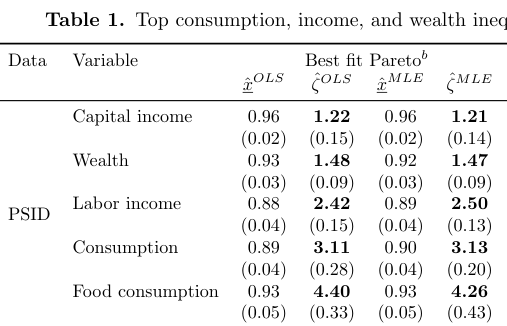
\includegraphics[width=0.9\linewidth]{figs_papers/gaillard_ranking_pareto_tails_data.png}
\end{figure}
                
    
\end{frame}


\begin{frame}{Theoretical results}
Using a continuous time HA model, they show that we need two key features to match this ranking:   
\begin{itemize}
    \item[1.] Non-homothetic preference for wealth
    \item[2.] Scale-dependent returns
\end{itemize}
(they also allow for random returns, death probability, progressive taxes)
\end{frame}

\begin{frame}{Quantitative model overview}
HA households with:
\begin{itemize}
    \item Idiosyncratic income shocks
    \item Scale dependent returns
    \item Type dependent returns
    \item Non-homothetic taste for wealth
\end{itemize}    
On the supply side, classic Cobb-Douglas production function with perfect competition.
\end{frame}

\begin{frame}{Quantitative results - Bellman equation}
$$\begin{aligned} V(y, z, a)= & \max _{c, a^{\prime} \geq a} \frac{c^{1-\gamma}}{1-\gamma}+\kappa \frac{(a / A)^{1-\nu}}{1-\nu} \\ &+\beta(1-\xi) \sum_{y^{\prime} \in \mathcal{Y}} \sum_{z^{\prime} \in \mathcal{Z}} P\left(y^{\prime} \mid y\right) P\left(z^{\prime} \mid z\right) V\left(y^{\prime}, z^{\prime}, a^{\prime}\right) \\ \text { s.t. } & c+a^{\prime}=w y-T(w y)+\left(1-\tau_K\right) r z S(a) a+a\end{aligned}$$    
with 
\begin{itemize}
    \item $y$ is the idiosyncratic productivity type 
    \item $\xi$ is the death probability
    \item $z$ is the idiosyncratic return type
    \item $T(wy)=wy - \frac{1-\tau_0}{1-\tau_L}(wy)^{1-\tau_L}$ (progressive taxations, HSV)
    \item $S(a)=1+\psi a^\eta$ (scale dependence)
\end{itemize}
\end{frame}

\begin{frame}{A note on death probability}
Many HA models with a Pareto tail have a death probability:
\begin{itemize}
    \item Main assumption: every period, households face a constant probability to die $\xi$
    \item They are replaced by new houeholds who start with zero wealth
    \item Because death is iid, does not add an extra state. But needs to change the forward step
    \item Key paper: perpetual youth model of Blanchard (1985) Yaari 
    
    \item Need to make assumptions on what happens to accidental bequests (paid to surviving households through annuity markets, taxes by governments, destroyed, etc)
\end{itemize}
$\to$ Especially important in non-homothetic model to have a non-degenerate distribution of wealth: we need a force to stop them from accumulating infinite amounts of wealth.
\end{frame}

\begin{frame}{Quantitative results - details on heterogeneous returns}

\vspace{1cm}
$z$ is a random variable that captures the return type:
\begin{itemize}
    
    \item $z\in(z_l,z_h)$, $z_l=1$, 'worker type', $z_h>1$, 'entrepreneur type'
    \item Follows a Markov chain: probability to become an entrepreneur is calibrated on data $q_{LH}=0.02$
    \item Probability to switch to worker type: $q_{HL}=0.2$
\end{itemize}
$\to$ as an entrepreneur, you want to save a lot because you get temporarily very high returns on your wealth.
    
\end{frame}

\begin{frame}{Quantitative results - supply side and market clearing}
\vspace{1cm}
Rest of the model is standard:
\begin{itemize}
    \item $Y=K^\alpha L^{1-\alpha}$, factors paid their marginal productivity
    \item Asset market clearing: $K=A=\int zS(a)adF(y,z,a)$
    \item Government budget balances (government fully taxes accidental bequests).
\end{itemize}
\end{frame}

\begin{frame}{Quantitative results - main exercise}

They calibrate most of the model parameters, and estimate:
\begin{itemize}
    \item[1.] $\kappa$: strength of taste for wealth
    \item[2.] $\nu$: exponent of the taste for wealth
    \item[3.] $z_h$: excess returns of high-return type
    \item[4.] $\psi$: strength of scale dependence
    \item[5.] $\eta$: exponent of scale dependence
\end{itemize}
\pause 
\pause And they target the following moments (at the steady-state)

\begin{itemize}
    \item[1.] Ratio of capital income / wealth Pareto coefficients 
    \item[2.] Ratio of consumption to wealth Pareto coefficients
    \item[3.] Ratio of wealth to labor income Pareto coefficients
\end{itemize}
+ Capital income to wealth tail for the top 1\% + W/Y=3.8 + Top 1\% wealth share
\end{frame}

\begin{frame}{Results}
\vspace{1cm}
\begin{figure}
        \centering
        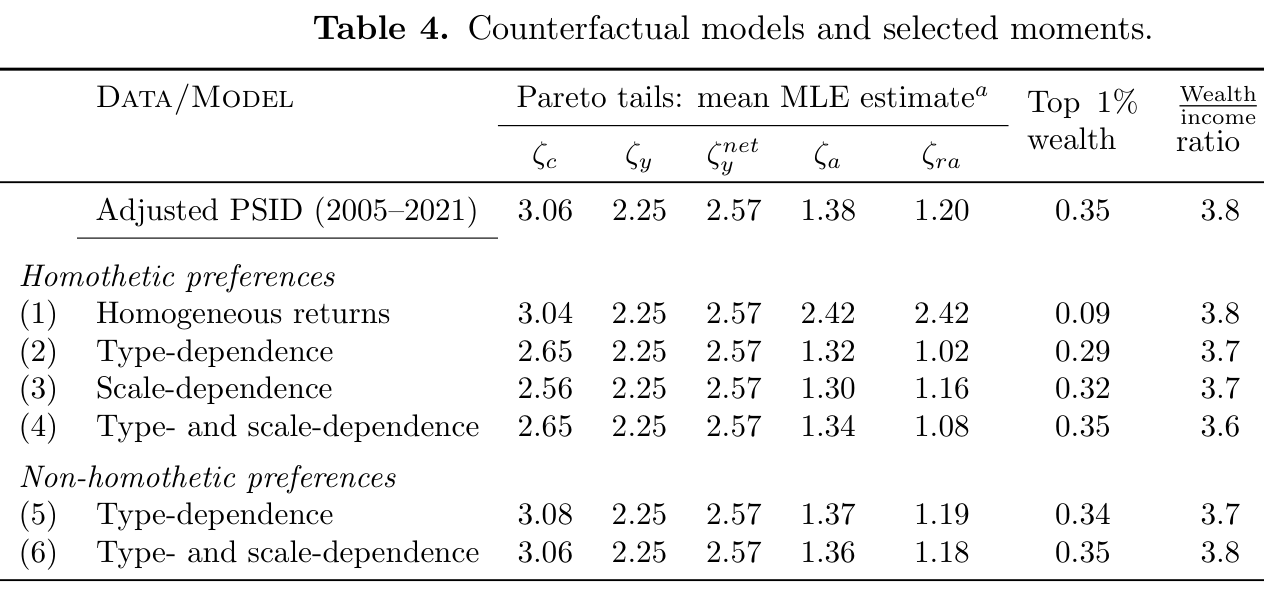
\includegraphics[width=\linewidth]{figs_papers/table_4_gaillard_results.png}
    \end{figure}
\pause 
$\to$ many models can generate high degree of wealth inequality. \pause \\ 
But both non-homothetic and type-dependence are key to match relative ranking of Pareto tails!
\end{frame}

\section{Hubmer, Krussel and Smith (2021) }
\begin{frame}{Explaining wealth inequality}
\begin{itemize}
\item Hubmer, Krussel and Smith (2021): \emph{Sources of US wealth inequality:
Past, present, and future}
\begin{itemize}
\item Model which matches key features of US wealth inequality in 1967
\item Can we account for changes in wealth inequality going forward from
1967 based on observables?
\begin{itemize}
\item I.e. changes in income inequality, taxes, asset returns 
\end{itemize}
\end{itemize}
\end{itemize}
\end{frame}
%
\begin{frame}{Model}
\begin{itemize}
\item <+->Household problem features non-linear tax schedules, heterogeneous
returns and $\beta$-het.
\begin{align*}
V_{t}(a_{t-1},p_{t},\beta_{t})= & \max_{a_{t+1}\geq0}\left\{ u(c_{t})+\beta_{t}\mathbb{E}[V_{t+1}(a_{t},p_{t+1},\beta_{t+1})|p_{t},\beta_{t}]\right\} \\
c_{t}+a_{t}= & y_{t}-\tau_{t}(y_{t})+(1-\tilde{\tau}_{t})\tilde{y}_{t}+T_{t}\\
y_{t}= & (\underline{r_{t}}+r_{t}^{X}\left(a_{t-1}\right))a_{t-1}+w_{t}l_{t}(p_{t})\\
\tilde{y}_{t} & =\sigma_{t}^{X}(a_{t-1})\eta_{t}a_{t-1}
\end{align*}
\item <+->Mean excess return $r_{t}^{X}\left(a_{t-1}\right)$
\begin{itemize}
\item How does mean returns vary with wealth?
\end{itemize}
\item <+->Standard deviation of excess returns: $\sigma_{t}^{X}\left(a_{t-1}\right)$
\begin{itemize}
\item How does return uncertainty vary with wealth?
\end{itemize}
\item <+->Example: If rich HHs primarily invest in stocks, poorer HHs in
bonds. Would expect both $r_{t}^{X}\left(a_{t-1}\right),\sigma_{t}^{X}\left(a_{t-1}\right)$
to be increasing in $a_{t-1}$
\end{itemize}
\end{frame}
%
\begin{frame}{Facts}
\begin{itemize}
\item Fagereng, Guiso, Malacrino, Pistaferri (2020) find that rates of returns
are:
\begin{itemize}
\item Heterogeneous across households (over 200 basis points between 10th
and 90th percentile of the distribution of returns)
\item Also heterogenous within asset classes
\begin{itemize}
\item So return differences cannot be explained only by poorer HHs holding
banket deposits and rich HHs investing in stocks
\end{itemize}
\item Persistent
\item Correlated with household wealth and across generations
\end{itemize}
\end{itemize}
\end{frame}
%
\begin{frame}

\frametitle{Equilibrium: capital market clearing}

\begin{wideitemize} 

\item <+->Need to find two equil. objects $(K_{t},\underline{r}_{t})$
for capital market clearing:
\begin{enumerate}
\item <+->aggregate capital (as usual) 
\[
K_{t}=\int a_{t}d\Gamma(a_{t})
\]
\item <+->aggregate capital income (redundant if $r_{t}^{X}(\cdot)=0$)
\begin{align*}
(MPK(K_{t})-\delta)K_{t} & =\int\left(\underline{r}_{t}+r_{t}^{X}(a_{t})\right)a_{t}d\Gamma(a_{t})
\end{align*}
\end{enumerate}
\item <+->Plus goods market clearing, but redundant given other
2

\end{wideitemize}
\end{frame}
%
\begin{frame}{Calibration strategy summary}
\begin{enumerate}
\item <+->Calibrate earnings process, tax rates, return process, social
safety net to observables
\item <+->Choose randomness in discount factor $\beta$ residually so as
to replicate the wealth distribution in the initial steady state (1967)
\item <+->Then feed in exogenous changes in tax rates, earnings inequality,
etc. between 1967 and 2015 to understand the role of these different
factors
\end{enumerate}
\end{frame}
%
\begin{frame}{Return heterogeneity}
\begin{itemize}
\item Overall return given asset holdings $a_{t-1}$ equals 
\begin{align*}
\underline{r}_{t}+r_{t}^{X}(a_{t-1})+\sigma^{X}(a_{t-1})\eta_{t}
\end{align*}
\item $\underline{r}_{t}$ is endogenous
\item $r_{t}^{X}(\cdot)$ and $\sigma^{X}(\cdot)$ are exogenous excess
return schedules (mean and st.dev.), taken from the data 
\item $\eta_{t}$ is an i.i.d. standard normal shock 
\item Reduced form portfolio choice 
\end{itemize}
\end{frame}
%
\begin{frame}

\frametitle{Calibration: return process}

\begin{align*}
r_{t}^{X}(a_{t})=\; & \sum_{c\in C}w_{c}(a_{t})\left(\bar{r}_{c,t}+\tilde{r}_{c}^{X}(a_{t})\right)\\
\sigma^{X}(a_{t})^{2}=\; & \sum_{c\in C}\left(w_{c}(a_{t})\tilde{\sigma}_{c}^{X}(a_{t})\right)^{2}
\end{align*}
\begin{itemize}
\item Asset classes $C$: risk-free, public equity, private equity, housing 
\item $\bar{r}_{c,t}$: aggregate return on asset class $c$ (U.S. data),
\textcolor{blue}{time-varying} 
\item Fixed over time, based on Swedish administrative data from Bach, Calvet,
Sodini (2016): 
\begin{itemize}
\item $w_{c}(\cdot)$: portfolio weights 
\item $\tilde{r}_{c}^{X}(\cdot)$: within asset class return heterogeneity 
\item $\tilde{\sigma}_{c}^{X}(\cdot)$: asset $c$ idiosyncratic return
standard deviation 
\end{itemize}
\end{itemize}
\end{frame}
%
\begin{frame}

\frametitle{Excess return schedule details}
\begin{itemize}
\item Aggregate Excess Returns in 1967 steady state: 
\begin{itemize}
\item public equity 0.067 (U.S., Kartashova 2014) 
\item private equity 0.129 (U.S., Kartashova 2014) 
\item housing 0.037 (incl. imputed rent; Jorda, et al, 2017) 
\end{itemize}
\vfill{}

\item and cross-sectional data from Bach, Calvet, Sodini (2019) implies 
\end{itemize}
 % Table generated by Excel2LaTeX from sheet 'r_ex_sd'  
\begin{table}[htbp]   
\centering 
\resizebox{1.1\textwidth}{!}{
  \begin{tabular}{lrrrrrrrrrrrrr}     \toprule           & \multicolumn{1}{l}{P0-P40} & \multicolumn{1}{l}{P40-P50} & \multicolumn{1}{l}{P50-P60} & \multicolumn{1}{l}{P60-P70} & \multicolumn{1}{l}{P70-P80} & \multicolumn{1}{l}{P80-P90} & \multicolumn{1}{l}{P90-P95} & \multicolumn{1}{l}{P95-P97.5} & \multicolumn{1}{l}{P97.5-P99} & \multicolumn{1}{l}{P99-P99.5} & \multicolumn{1}{l}{P99.5-P99.9} & \multicolumn{1}{l}{P99.9-P99.99} & \multicolumn{1}{l}{Top 0.01\%} \\     \midrule     \multicolumn{5}{l}{fixed portfolio weights} &       &       &       &       &       &       &       &       &  \\ \cmidrule{1-5}    risk-free  & 0.722 & 0.412 & 0.248 & 0.182 & 0.156 & 0.134 & 0.115 & 0.102 & 0.090 & 0.079 & 0.071 & 0.051 & 0.029 \\     housing & 0.162 & 0.394 & 0.580 & 0.662 & 0.678 & 0.674 & 0.658 & 0.626 & 0.572 & 0.482 & 0.363 & 0.253 & 0.155 \\     public equity & 0.113 & 0.189 & 0.165 & 0.147 & 0.153 & 0.170 & 0.189 & 0.207 & 0.219 & 0.232 & 0.230 & 0.185 & 0.179 \\     private equity & 0.002 & 0.005 & 0.007 & 0.009 & 0.013 & 0.021 & 0.038 & 0.065 & 0.118 & 0.207 & 0.336 & 0.511 & 0.637 \\     \midrule     \bottomrule     \end{tabular}% 
} 
\end{table}%
\end{frame}
%
\begin{frame}

\frametitle{Schedule of excess returns}

\begin{figure}
\centering 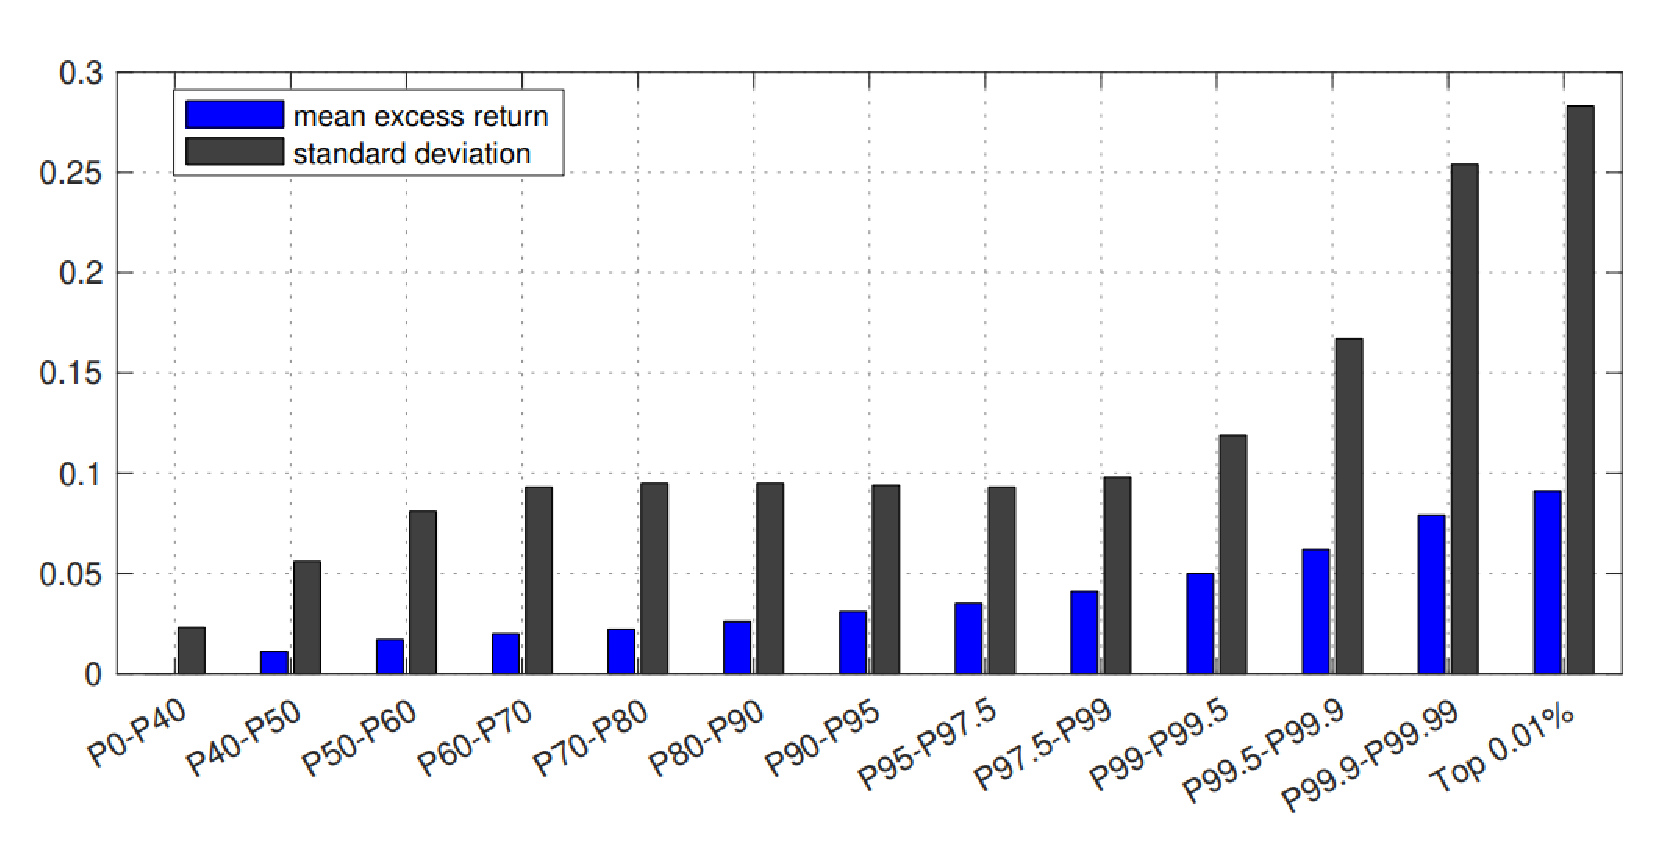
\includegraphics[width=1\textwidth]{HKS-Figs/4} {\footnotesize{
\caption*{Data sources: Bach, Calvet, Sodini (2019); Kartashova (2014); Jorda,
Knoll, Kuvshinov, Schularick, Taylor (2019); Case-Shiller.}
}}
\end{figure}
\end{frame}

\subsection{Results}
\begin{frame}{Results, I: Steady state (1967)}
\begin{itemize}
\item Steady state fit (with and without $\beta$-het)
\end{itemize}
\begin{table}[htbp]   
\centering 
\resizebox{\textwidth}{!}{      
\begin{tabular}{lrrrr}     \toprule           
& Top 10\% & Top 1\% & Top 0.1\% & Top 0.01\% \\     
\midrule     
Data & 70.8\% & 27.8\% & 9.4\% & 3.1\% \\
Single-$\beta$ Model & 66.6\% & 23.7\% & 11.2\% & 7.2\% \\
Benchmark Model & 73.8\% & 27.4\% & 8.4\% & 3.2\% \\     \midrule           & Bottom 50\% & Fraction $a<0$ &       &  \\  
  \midrule     
Data & 4.0\% & 8.0\% &       &  \\     
Single-$\beta$ Model & 3.5\% & 7.3\% &       &  \\     
Benchmark Model & 3.0\% & 6.6\% &       &  \\     
\bottomrule     
\end{tabular}}% 
\end{table}%
\end{frame}
%
\begin{frame}{Results, I: steady state (1967)}

\begin{figure}[H]     \centering     
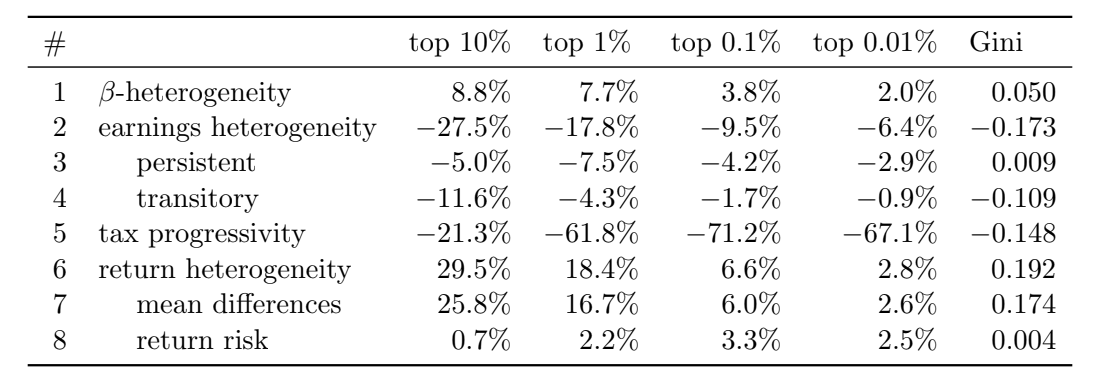
\includegraphics[width=0.85\linewidth]{HKS-Figs/table2.png}     
\end{figure}
\begin{itemize}
\item How to read: Shutting of $\beta$-het reduces top 10\% wealth share
by 8.8\% 
\item Model matches wealth distribution well on its entire domain 
\begin{itemize}
\item return heterogeneity is key ingredient 
\item wealth concentration is mitigated by progressive taxation and labor
income risk 
\end{itemize}
\end{itemize}
\end{frame}
%
\begin{frame}

\frametitle{Next step: transition}

The authors feed in four different factors that have changed during
the past 50 years \begin{wideitemize} 

\item Decrease in tax progressivity 

\item Increase in labor income risk 

\item Increase in income going to the top 

\item Changing return premia to different asset classes 

\end{wideitemize} 
\end{frame}
%
\begin{frame}

\frametitle{Observed change 1: Decrease in tax progressivity}
\begin{itemize}
\item Federal effective tax rates (Piketty \& Saez 2007): income, payroll,
corporate and estate taxes 
\end{itemize}
\begin{figure}[htbp]
\centering 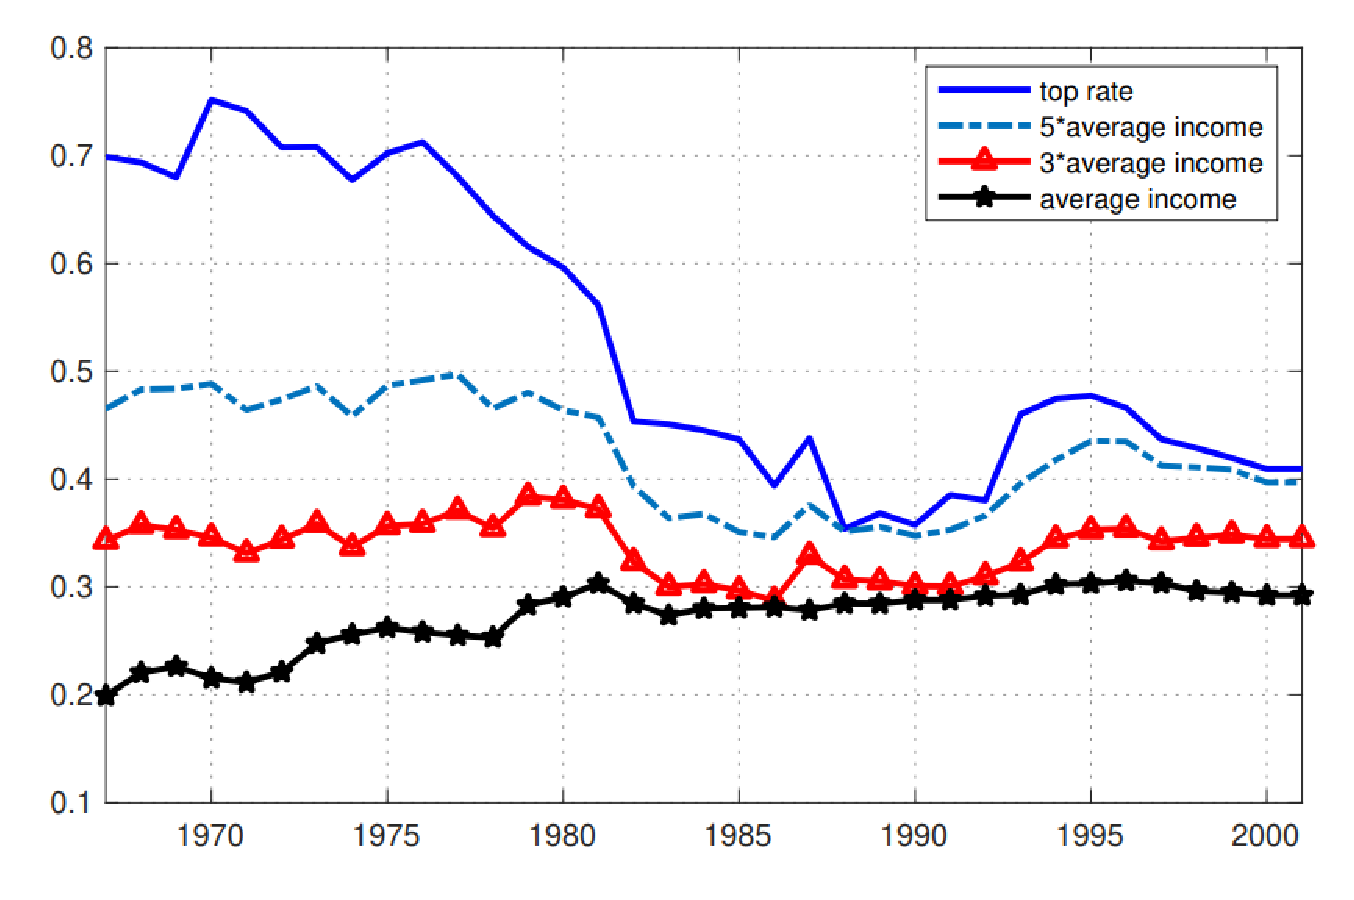
\includegraphics[width=0.8\textwidth]{HKS-Figs/5}
\end{figure}
\end{frame}
%
\begin{frame}

\frametitle{Observed change 2: Increase in labor income risk}
\begin{itemize}
\item Estimates for variance of persistent and temporary components 1967-2000
(Heathcote, Storesletten \& Violante 2010) 
\end{itemize}
\begin{figure}[htbp]
\centering 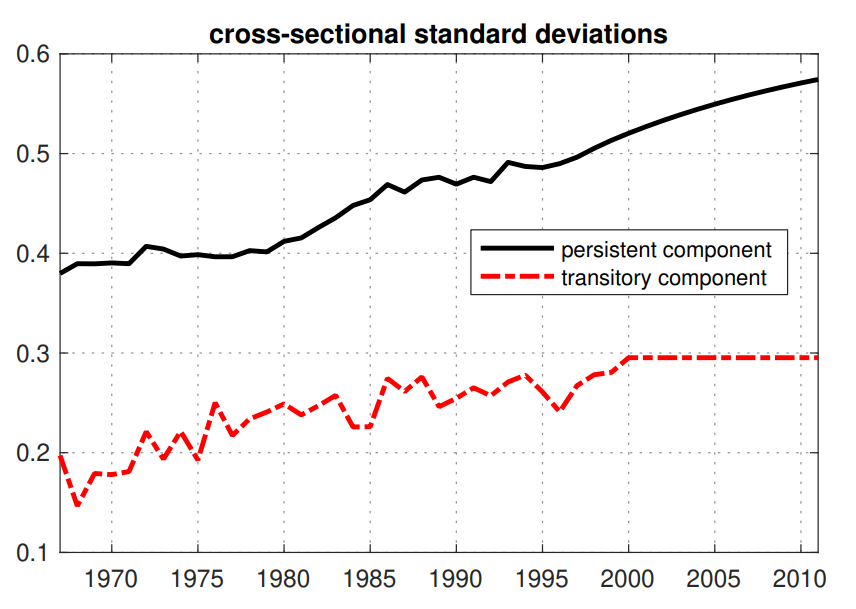
\includegraphics[width=0.8\textwidth]{HKS-Figs/6}
\end{figure}
\end{frame}
%
\begin{frame}

\frametitle{Observed change 3: Increase in top labor income shares}
\begin{itemize}
\item Adjust standard AR(1) in idiosyncratic productivity by imposing a
Pareto tail for the top 10\% earners: calibrated tail coefficient
decreases from 2.8 to 1.9 (updated Piketty \& Saez 2003 series) 
\end{itemize}
\begin{figure}[htbp]
\centering 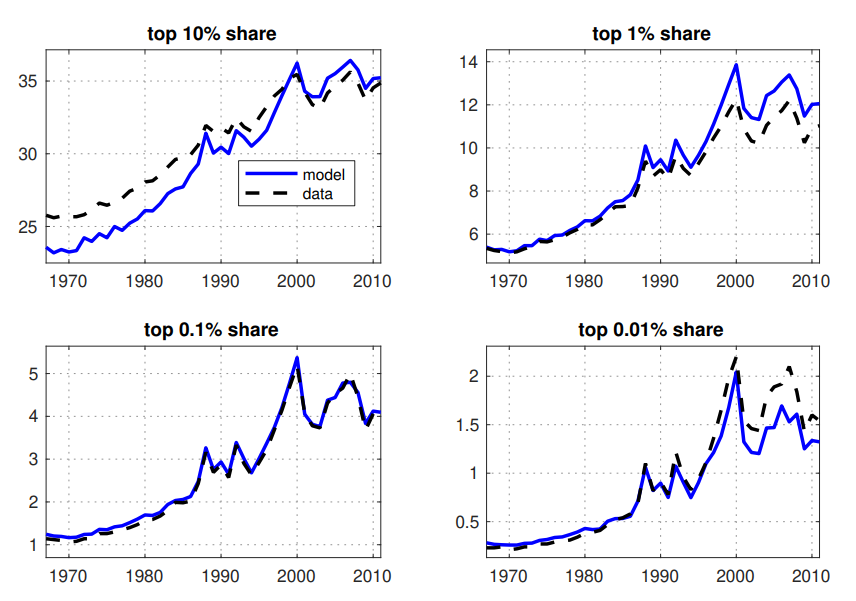
\includegraphics[width=0.8\textwidth]{HKS-Figs/7}
\end{figure}
\end{frame}
%
\begin{frame}

\frametitle{Observed change 4: return premia}

\begin{wideitemize} 

\item Feed in (smoothed) time series of aggregate U.S. asset premia
(Kartashova 2014, Case-Shiller index) \end{wideitemize} \visible<2->{ 
\begin{figure}[htbp]
\centering 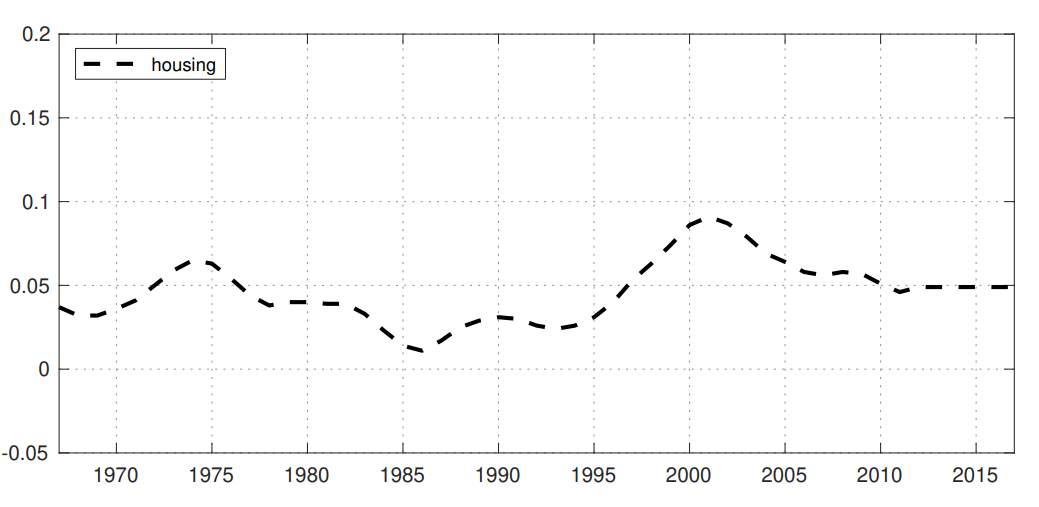
\includegraphics[width=1\textwidth]{HKS-Figs/8}
\end{figure}
} 
\end{frame}
%
\begin{frame}

\frametitle{Observed change 4: return premia}

\begin{wideitemize} 

\item feed in (smoothed) time series of aggregate U.S. asset premia
(Kartashova 2014, Case-Shiller index) \end{wideitemize} 
\begin{figure}[htbp]
\centering 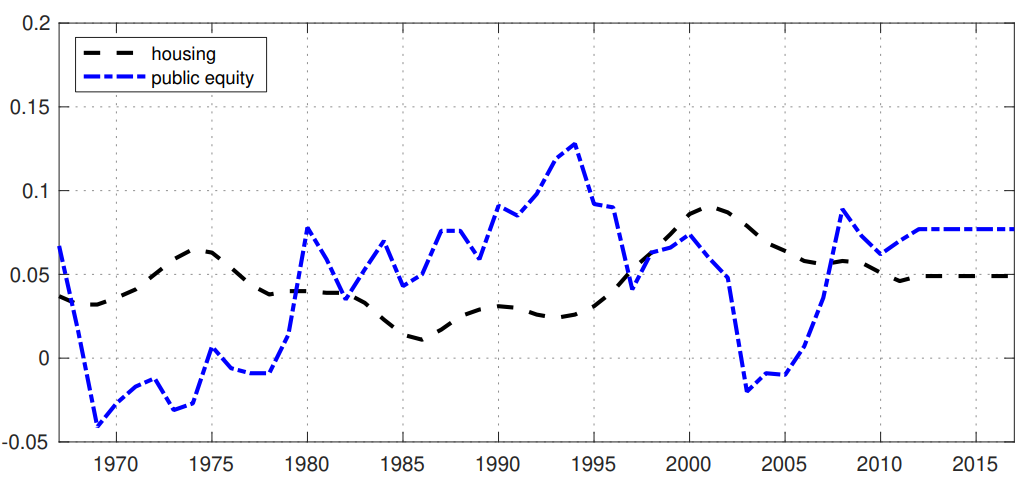
\includegraphics[width=1\textwidth]{HKS-Figs/9}
\end{figure}
\end{frame}
%
\begin{frame}

\frametitle{Observed change 4: return premia}

\begin{wideitemize} 

\item feed in (smoothed) time series of aggregate U.S. asset premia
(Kartashova 2014, Case-Shiller index) 

\end{wideitemize} 
\begin{figure}[htbp]
\centering 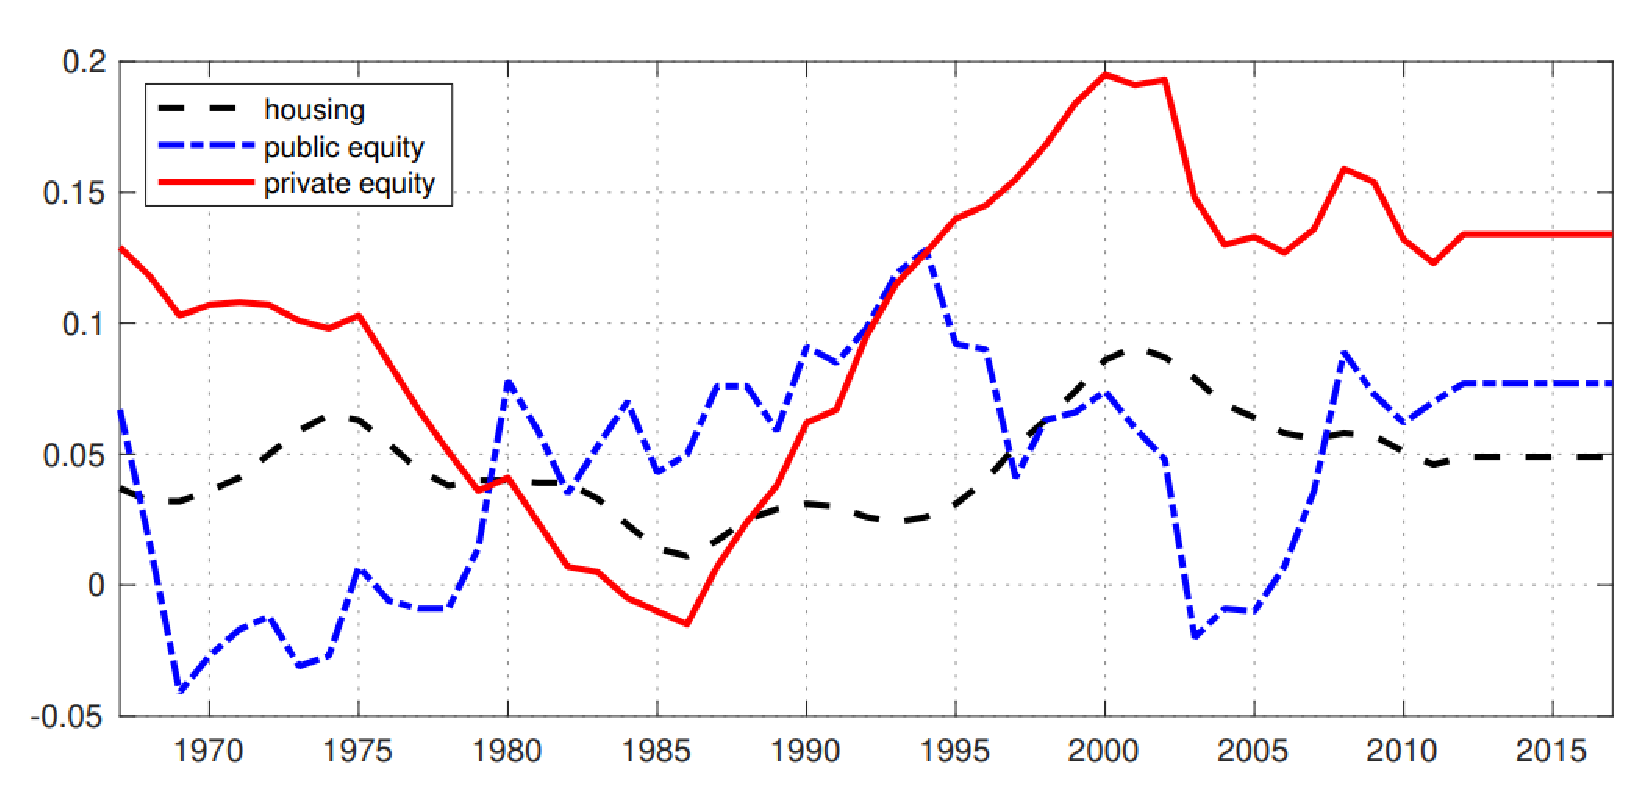
\includegraphics[width=1\textwidth]{HKS-Figs/10}
\end{figure}
\end{frame}
%
\begin{frame}

\frametitle{Results, II: historical evolution}

\begin{figure}[htbp]
\centering \includegraphics[width=1\textwidth]{HKS-Figs/fig8_color}
\end{figure}
\end{frame}
%
\begin{frame}

\frametitle{Results: Capital-output ratio and bottom 50 \%}

\begin{figure}[htbp]
\centering 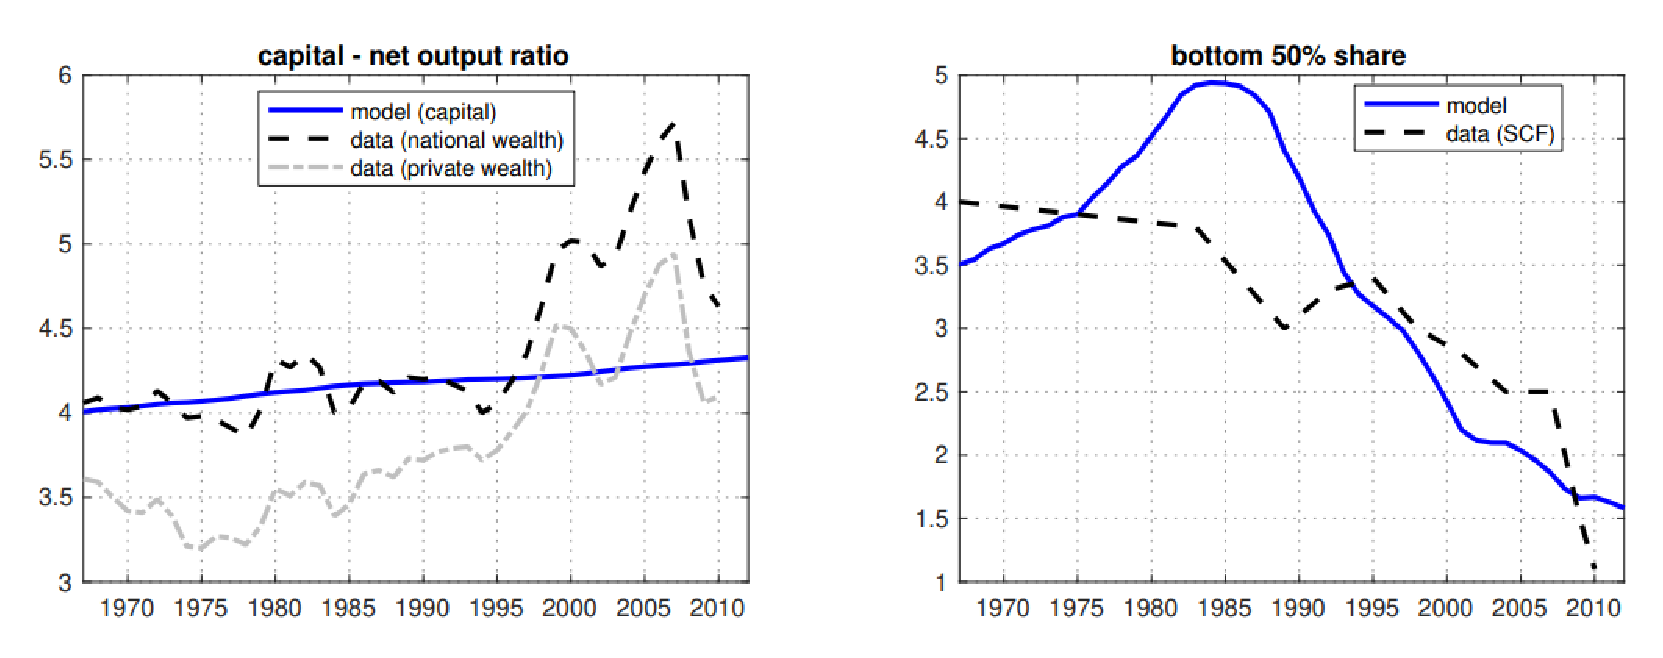
\includegraphics[width=1\textwidth]{HKS-Figs/12}
\end{figure}
\end{frame}
%
\begin{frame}

\frametitle{Results: Risk-free rate}
\begin{itemize}
\item Return premia are matched in model by construction 
\item Risk-free rate $r$ is endogenous: comparable level and decline 
\end{itemize}
\begin{figure}[htbp]
\centering 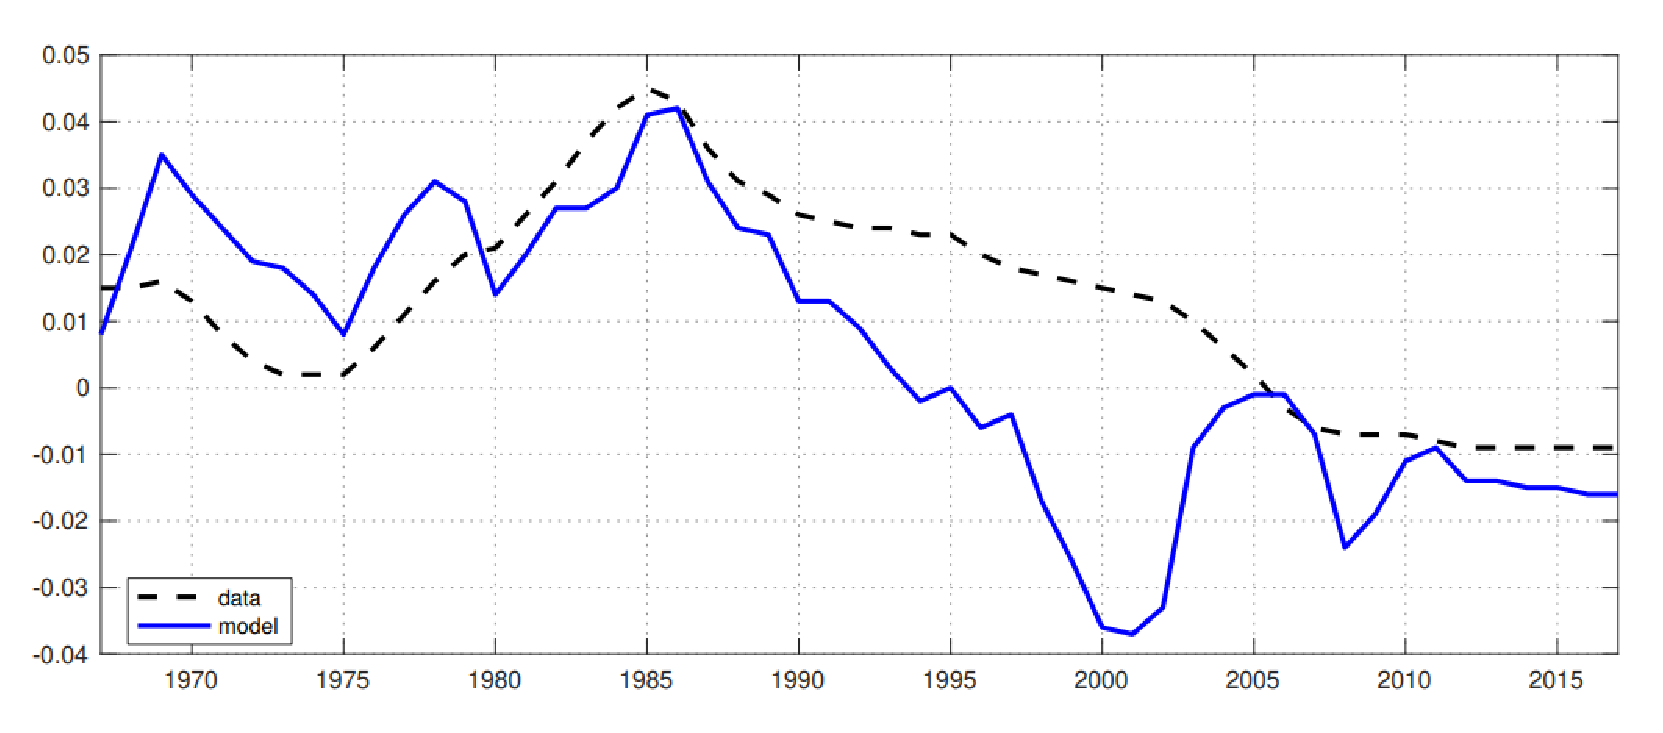
\includegraphics[width=1\textwidth]{HKS-Figs/13}
\end{figure}
\end{frame}
%
\begin{frame}

\frametitle{Decomposition of transitional dynamics}

\begin{figure}[htbp]
\centering 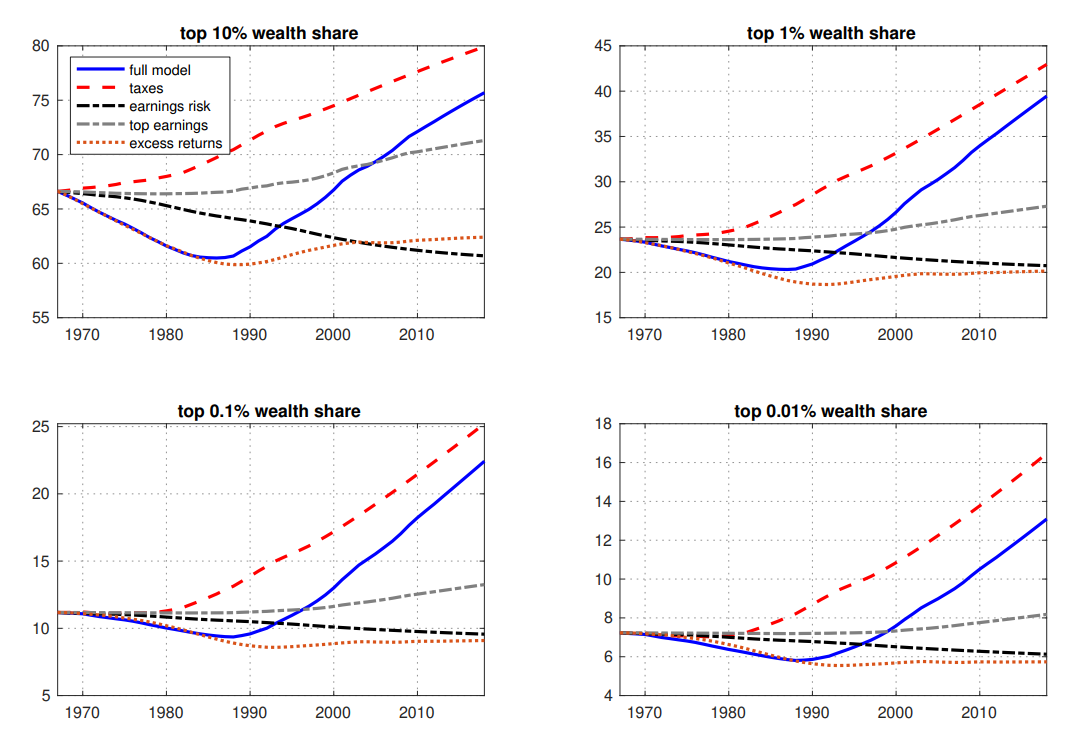
\includegraphics[width=1\textwidth]{HKS-Figs/14}
\end{figure}
\end{frame}
%
\begin{frame}[label=decomposemain]

\frametitle{Decomposition of transitional dynamics}

\begin{wideitemize} 

\item Overall increase in wealth inequality (more than) fully explained
by declining tax progressivity 
\begin{itemize}
\item Primarily due to direct effect on resource distribution and not due
to changing savings behavior 
\end{itemize}
\item Time-varying return premia account for U-shape in wealth inequality 

\item Subtle role of increasing earnings dispersion 
\begin{itemize}
\item Thickening Pareto tail in labor income contributes slightly positively
to wealth inequality 
\item Increase in overall earnings risk \emph{decreases} wealth inequality
because precautionary savings motive is stronger for poorer HHs
\end{itemize}
\end{wideitemize}
\end{frame}
%
\begin{frame}{Summary}
\begin{itemize}
\item \textbf{Hubmer, Krussel and Smith (2021)}
\item HANC with:
\begin{itemize}
\item Income risk
\item Return heterogeneity 
\item $\beta$-heterogeneity
\item Tax system 
\end{itemize}
\item Main finding: 
\begin{itemize}
\item Return heterogeneity key in matching initial (1967) wealth inequality
\item Can roughly explain evolution in US wealth inequality with observable
changes in tax systems 
\end{itemize}
\end{itemize}
\end{frame}
%
\begin{frame}{Ozkan et al. (2024)}
\begin{itemize}
\item <+->Ozkan et al. (2024) takes a \emph{lifecycle perspective}:
\begin{itemize}
\item Why do some people become wealther than others?
\item Use detailed Norwegian admin data
\end{itemize}
\item <+->Evaluate contribution from
\begin{enumerate}
\item Inheritances (bequests) $H_{it}$
\item Return heterogeneity $r_{it}$
\item Saving rate heterogeneity $s_{it}$
\item Labor earnings $L_{it}$
\item Initial wealth $a_{i0}$
\end{enumerate}
\item <+->Using budget constraint:
\[
a_{it}=a_{it-1}+\left(L_{it}+H_{it}+r_{it}a_{it-1}\right)\times s_{it}
\]
\end{itemize}
\end{frame}
%
\begin{frame}{Results from Ozkan et al. (2024)}
\begin{itemize}
\item Left panel: Decomposition of wealth for top 0.1\%
\item Right panel: >>Poorest<< HHs \emph{within} top 0.1\% \emph{(New
Money}) \vspace{1cm}\\
\begin{figure}[H]     \centering     
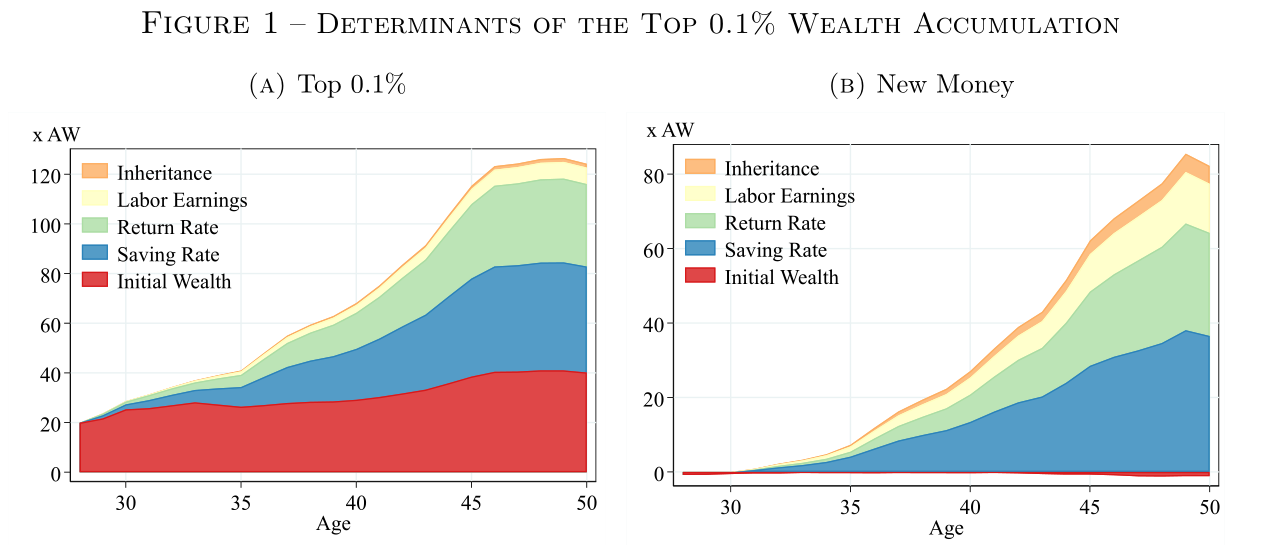
\includegraphics[width=0.85\linewidth]{figs_papers/Ozkan_et_al_2024_fig1.png}     
\end{figure}
\end{itemize}
\end{frame}

\section{Application to Wealth Taxation}
\begin{frame}{Wealth taxation I}
\begin{itemize}
\item Spend a lot of time understanding \emph{what} drives wealth inequality 
\item <+->We will now see an application where the specific source of inequality
matters
\item <+->\textbf{Wealth taxation}
\begin{itemize}
\item <+->Why would we want to tax wealth?
\begin{itemize}
\item <+-|handout:0> Redistribution: Transfer from HHs with low MUC to
HHs with high MUC \emph{raises }aggregate welfare
\end{itemize}
\item <+->Why not?
\begin{itemize}
\item <+-|handout:0> Efficiency concern 1: Wealthy households might be
more productive - do not want to distort their labor supply/investments
\item <+-|handout:0> Efficiency concern 2: In the Ramsey model aggregate
K is generally below the golden rule level 
\end{itemize}
\end{itemize}
\end{itemize}
\end{frame}
%
\begin{frame}{Wealth taxation II}
\begin{itemize}
\item Guvenen et al. (2023): \emph{Use It or Lose It: Efficiency and Redistributional
Effects of Wealth Taxation}
\item <+->Study optimal taxation in two tax systems:
\begin{itemize}
\item Wealth tax: $a_{i}$
\item Capital income tax : $r\times a_{i}$
\end{itemize}
\item <+->Note: Without return heterogeneity two tax system are equivalent
\begin{itemize}
\item After tax wealth /w CI tax : $a_{i}+\left(1-\tau_{k}\right)ra_{i}$
\item After tax wealth /w wealth tax : $\left(1-\tau_{a}\right)a_{i}+ra_{i}$
\end{itemize}
\item <+->Social planner can implement same allocation using these two
different instruments by setting $\tau_{a}=r\tau_{k}$
\end{itemize}
\end{frame}
%
\begin{frame}{Taxation with return heterogeneity}
\begin{itemize}
\item <+->What if returns differ across agents, $r_{i}?$
\begin{itemize}
\item No equivalence between tax systems
\end{itemize}
\item <+->With capital income taxation:
\begin{itemize}
\item A highly productive agent (high $r_{i}$) will be taxed more than
less productive agents (low $r_{i}$)
\begin{itemize}
\item Tax burden falls proportinally more on productive agents $\Rightarrow$distortionary
\end{itemize}
\end{itemize}
\item <+->With wealth taxation:
\begin{itemize}
\item All agents with same wealth pay same tax regardless of return $r_{i}$
\item Shifts tax base towards unproductive agents 
\end{itemize}
\item <+->Note: We say HHs with high $r_{i}$ are more \textbf{productive }
\begin{itemize}
\item Think in terms of \emph{entrepreneurial} models
\item High productivity HHs have better technology (i.e. are better entrepreneurs)
and can make their wealth growth faster (high $r_{i}$)
\end{itemize}
\end{itemize}
\end{frame}
%
\begin{frame}{Model}
\begin{itemize}
\item <+->HH problem:
\[
\max_{\left\{ c_{t}\right\} _{t=0}^{T}}E\sum_{t=0}^{T}\beta^{t}\left(s_{t}\frac{c_{t}^{1-\sigma}}{1-\sigma}+\left(1-s_{t}\right)\phi\left(a_{t}\right)\right)
\]
\[
a_{t}+c_{t}=\mathcal{W}\left(a_{t-1},z_{t-1}\right)+w_{t}\left(e_{t}\right)\ell_{t},\quad a_{t}\geq\underline{a}
\]
\[
\mathcal{W}\left(a_{t-1},z_{t}\right)=\begin{cases}
\begin{array}{c}
a_{t-1}+\left(\pi\left(a_{t-1},z_{t}\right)+ra_{t-1}\right)\left(1-\tau_{k}\right)\\
a_{t-1}\left(1-\tau_{a}\right)+\left(\pi\left(a_{t-1},z_{t}\right)+ra_{t-1}\right)
\end{array} & \begin{array}{c}
\text{if CI tax}\\
\text{if wealth tax}
\end{array}\end{cases}
\]
\item <+->Entrepreneurial abilitiy $z$ follow markov chain with values
$z=\left[0,z_{L},z_{H}\right]'$ and transition matrix $\Pi_{z}$
\begin{itemize}
\item HHs with $z=0$ are normal workers
\item HHs with $z=z_{L}$ are >>unproductive<< entrepreneurs 
\item HHs with $z=z_{H}$ are >>productive<< entrepreneurs 
\end{itemize}
\item <+->Entrepreneurial profit $\pi\left(a_{t-1},z_{t-1}\right)$ given
by:
\[
\pi\left(a_{t-1},z_{t}\right)=\max_{k_{t}<\kappa a_{t-1}}\left\{ p_{t}z_{t}k_{t}-\left(r+\delta\right)k_{t}\right\} 
\]
\end{itemize}
\end{frame}
%
\begin{frame}{Empirical fit}
\begin{itemize}
\item Calibrate model to US. Model reproduces wealth inequality in the data,
also for the extremely rich\\
\begin{figure}[H]     \centering     
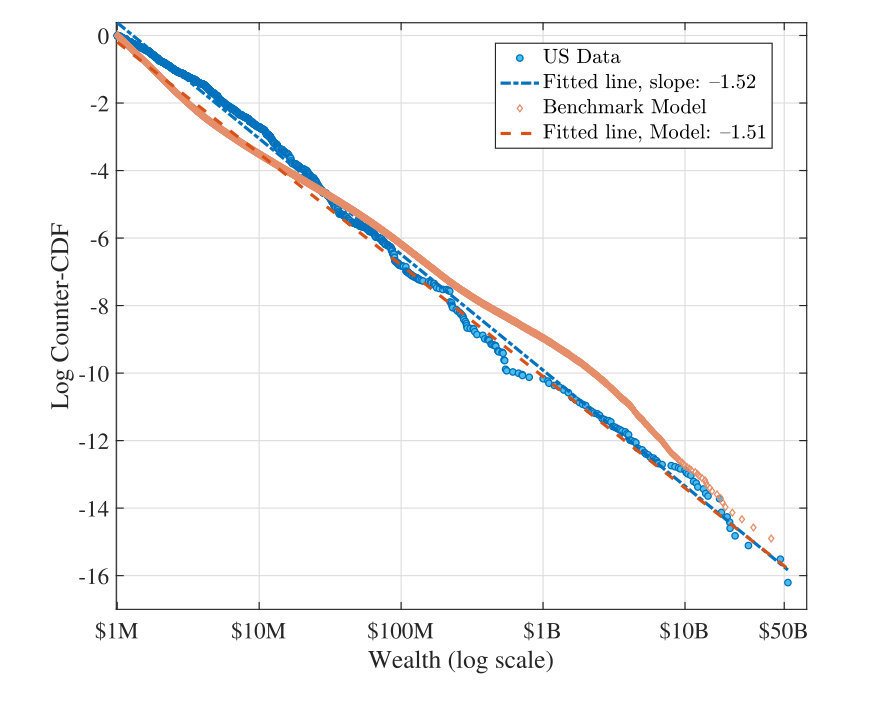
\includegraphics[width=0.7\linewidth]{figs_papers/Guvenen_et_al_2023_pareto.png}     
\end{figure}
\end{itemize}
\end{frame}
%
\begin{frame}{Results}
\begin{itemize}
\item Exercise: Replace capital income tax $\tau_{k}=25\%$ with wealth
tax $\tau_{a}>0$ in a government revenue-neutral way (requires $\tau_{a}=1.2\%$)\\
\begin{figure}[H]     \centering     
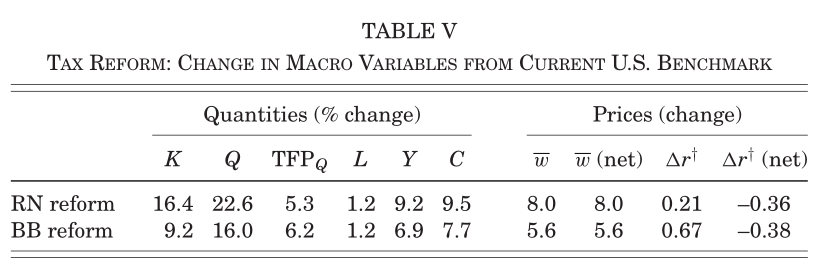
\includegraphics[width=0.85\linewidth]{figs_papers/Guvenen_et_al_2023_tableV.png}     
\end{figure}
\item Capital, productivity output, consumption, wages increases 
\begin{itemize}
\item Efficency gain from shifting tax base away from productive agents 
\end{itemize}
\item Also generates large welfare gain (around 7\% consumption equivalent
gains)
\end{itemize}
\end{frame}
%
\begin{frame}{Results - optimal taxation}
\begin{itemize}
\item Now find tax rates that maximize aggregate welfare
\begin{itemize}
\item Wealth taxation (OWT) vs. capital income taxation (OKIT)
\end{itemize}
\item Results:\\
\begin{figure}[H]     \centering     
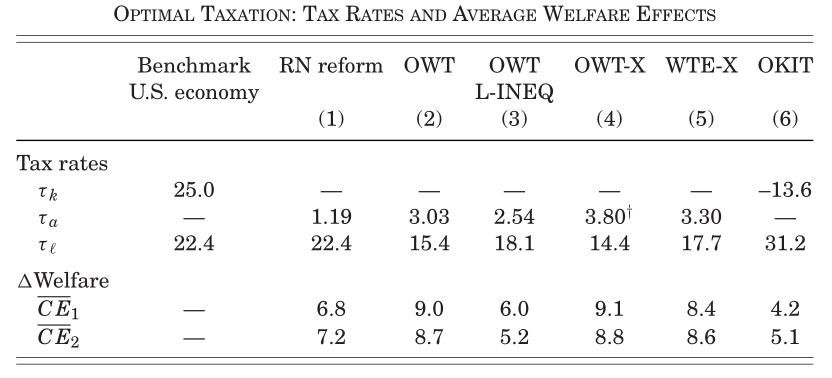
\includegraphics[width=0.85\linewidth]{figs_papers/Guvenen_et_al_2023_tableVII.png}     
\end{figure}
\item Wealth taxation: Positive taxation $\tau_{a}=3.03\%$, large welfare
gain of $9\%$
\item Capital income taxation: \emph{Subsidy $\tau_{K}=-13.6\%$ }and smaller
welfare gain of $4.2\%$
\end{itemize}
\end{frame}
%
\begin{frame}{Summary}
\begin{itemize}
\item <+->Guvenen et al. (2023) study optimal wealth taxation 
\item <+->Source of wealth inequality matters for optimal taxation 
\item <+->If driven by return heterogeneity \textbf{wealth tax }strongly
preffered to \textbf{capital income tax }
\begin{itemize}
\item Why? It distorts investment decisions of high productivity HHs less
than a capital income tax
\end{itemize}
\end{itemize}

\end{frame}

\section{Exercise}
\begin{frame}{Standard HANC model with return heterogeneity}
\begin{itemize}
\item HH problem:
\begin{align*}
v_{t}(,e_{it}r_{it}^{x},,a_{it-1}) & =\max_{c_{t}}u(c_{t})+\beta\underline{v}_{t+1}(e_{it+1},r_{it+1}^{x},a_{it})\\
 & \text{s.t.}\\
a_{it} & =(1+r_{t}+r_{it}^{x})a_{it-1}+w_{t}e_{it}-c_{it}\\
\log e_{it+1} & =\rho_{e}\log e_{it}+\psi_{it+1}^{e},\quad\psi_{it+1}^{e}\sim\mathcal{N}\left(0,\sigma_{e}^{2}\right)\\
r_{it+1}^{x} & =\overline{r}^{x}+\rho_{z}r_{it}^{x}+\psi_{it+1}^{r^{x}},\quad\psi_{it+1}^{r^{x}}\sim\mathcal{N}\left(0,\sigma_{r^{x}}^{2}\right)\\
a_{it} & \geq0
\end{align*}
\item \textbf{Q1}:\textbf{ }Solve the PE HA model with return heterogeneity
\item \textbf{Q2}: Calibrate the HANC model such that average returns are
4\%
\item \textbf{Q3}: Calibrate a standard HA model without return heterogeneity.
Compare the wealth distributions obtained in the two models.
\end{itemize}
\end{frame}
%

\section{Summary}
\begin{frame}{Summary and next week}
\begin{itemize}
\item \textbf{Today: }Various explanations of wealth inequality
\begin{enumerate}
\item Preferences
\item Bequests
\item Returns 
\end{enumerate}
\item \textbf{Next week: }Secular stagnation 
\item \textbf{Midterm evaluation: } Don't forget to fill out questionnaire 
\item \textbf{Homework exercise}: Solve model with return heterogeneity
\begin{itemize}
\item See Github repo 
\end{itemize}
\end{itemize}
\end{frame}
%

\end{document}
